\documentclass[11pt,a4paper]{article}

% ========== PACKAGES ==========
\usepackage[utf8]{inputenc}
\usepackage[T1]{fontenc}
\usepackage{lmodern}
\usepackage[margin=1in]{geometry}
\usepackage{graphicx}
\usepackage{xcolor}
\usepackage{titlesec}
\usepackage{enumitem}
\usepackage{hyperref}
\usepackage{fancyhdr}
\usepackage{tabularx}
\usepackage{booktabs}
\usepackage{fontawesome5}
\usepackage{tcolorbox}
\usepackage{tikz}
\usepackage{setspace}

% ========== COLORS ==========
\definecolor{primary}{RGB}{16, 185, 129}    % Emerald Green
\definecolor{secondary}{RGB}{10, 10, 10}    % Pure Black
\definecolor{accent}{RGB}{239, 68, 68}      % Red
\definecolor{darkbg}{RGB}{13, 13, 13}
\definecolor{textgray}{RGB}{156, 163, 175}

% ========== STYLING ==========
\hypersetup{
    colorlinks=true,
    linkcolor=primary,
    urlcolor=primary,
    pdfauthor={Priyanshu},
    pdftitle={iStocks - AI-Powered Stock Analysis Platform}
}

\titleformat{\section}{\Large\bfseries\color{primary}}{\thesection}{1em}{}
\titleformat{\subsection}{\large\bfseries\color{black}}{\thesubsection}{1em}{}
\titleformat{\subsubsection}{\normalsize\bfseries\color{textgray}}{\thesubsubsection}{1em}{}

\pagestyle{fancy}
\fancyhf{}
\fancyhead[L]{\textcolor{textgray}{\small iStocks Documentation}}
\fancyhead[R]{\textcolor{textgray}{\small \thepage}}
\renewcommand{\headrulewidth}{0.5pt}
\renewcommand{\headrule}{\hbox to\headwidth{\color{primary}\leaders\hrule height \headrulewidth\hfill}}

\setlength{\parindent}{0pt}
\setlength{\parskip}{8pt}

% ========== CUSTOM BOX ==========
\newtcolorbox{featurebox}[1][]{
    colback=primary!5,
    colframe=primary,
    fonttitle=\bfseries,
    title=#1,
    rounded corners,
    boxrule=1pt,
    left=8pt,
    right=8pt,
    top=6pt,
    bottom=6pt
}

\newtcolorbox{techbox}[1][]{
    colback=gray!5,
    colframe=gray!50,
    fonttitle=\bfseries,
    title=#1,
    rounded corners,
    boxrule=0.5pt
}

% ========== DOCUMENT ==========
\begin{document}

% ========== TITLE PAGE ==========
\begin{titlepage}
    \centering
    \vspace*{2cm}
    
    % Logo representation
    
\begin{tikzpicture}
        \fill[primary, rounded corners=8pt] (0,0) rectangle (2,2);
        \draw[white, ultra thick, ->, >=stealth] (0.3,0.5) -- (1,1.5) -- (1.7,0.8);
    \end{tikzpicture}
    
    \vspace{1cm}
    
    {\Huge\bfseries\textcolor{primary}{iStocks}}\\[0.5cm]
    {\Large\textcolor{textgray}{AI-Powered Stock Analysis Platform}}
    
    \vspace{2cm}
    
    \rule{0.6\textwidth}{1pt}
    
    \vspace{2cm}
    
    {\large\textbf{Technical Documentation \& Feature Overview}}\\[0.3cm]
    {\normalsize Version 1.0}
    
    \vspace{3cm}
    
    {\normalsize\textcolor{textgray}{A comprehensive intelligent stock analysis platform\\combining real-time market data with AI-driven insights}}
    
    \vfill
    
    {\small\textcolor{textgray}{January 2026}}\\[0.5cm]
    {\normalsize Live at: \textcolor{primary}{\url{https://istocks.codes}}}
    
\end{titlepage}

% ========== TABLE OF CONTENTS ==========
\tableofcontents
\newpage

% ========== EXECUTIVE SUMMARY ==========
\section{Executive Summary}

\textbf{iStocks} is a cutting-edge financial technology platform designed to democratize institutional-grade stock analysis for retail investors in the Indian market. The platform combines real-time market data from NSE/BSE with advanced AI capabilities powered by Google's Gemini model to deliver actionable investment insights.

\begin{featurebox}[Key Value Propositions]
\begin{itemize}[leftmargin=*]
    \item \textbf{AI-Driven Analysis:} Natural language queries to understand complex market dynamics
    \item \textbf{Real-Time Data:} Live stock prices and technical indicators
    \item \textbf{Strategy Repository:} Create, backtest, and share trading strategies
    \item \textbf{Technical Analysis:} 20+ indicators including RSI, MACD, Bollinger Bands
    \item \textbf{Zero Cost Barrier:} Free access to professional-grade tools
\end{itemize}
\end{featurebox}

% ========== PLATFORM FEATURES ==========
\section{Platform Features}

\subsection{AI-Powered Chatbot}

The heart of iStocks is its intelligent conversational AI assistant that understands financial queries in natural language.

\textbf{Capabilities:}
\begin{itemize}[leftmargin=*]
    \item \textbf{Natural Language Processing:} Ask questions like ``How is Reliance performing?'' or ``Compare TCS vs Infosys''
    \item \textbf{Technical Analysis Interpretation:} Explains RSI, MACD, and other indicators in simple terms
    \item \textbf{Pattern Recognition:} Identifies bullish/bearish patterns and trends
    \item \textbf{Multi-Stock Comparison:} Compare multiple stocks simultaneously
    \item \textbf{Volume Analysis:} Analyzes trading volumes and identifies unusual activity
\end{itemize}

\textbf{AI Model:} Google Gemini 2.5 Pro - chosen for its superior reasoning capabilities and context understanding.

\subsection{Real-Time Stock Dashboard}

\begin{featurebox}[Dashboard Components]
\begin{tabularx}{\textwidth}{lX}
    \textbf{Price Card} & Live price, change percentage, high/low with color-coded indicators \\
    \textbf{Interactive Chart} & Candlestick and line charts with zoom, pan capabilities \\
    \textbf{Technical Panel} & 20+ indicators with visual representations \\
    \textbf{Insights Panel} & AI-generated analysis and recommendations \\
\end{tabularx}
\end{featurebox}

\subsection{Technical Indicators}

The platform calculates and displays comprehensive technical indicators:

\begin{table}[h]
\centering
\begin{tabular}{ll}
\toprule
\textbf{Category} & \textbf{Indicators} \\
\midrule
Moving Averages & SMA (20, 50, 200), EMA (12, 26) \\
Momentum & RSI, Stochastic Oscillator, Williams \%R, ROC \\
Trend & MACD, ADX, Plus/Minus DI \\
Volatility & Bollinger Bands (Upper, Middle, Lower), ATR \\
Volume & OBV (On-Balance Volume), Volume Analysis \\
Others & CCI (Commodity Channel Index) \\
\bottomrule
\end{tabular}
\caption{Technical Indicators Available on iStocks}
\end{table}

\subsection{Sangraha - Strategy Repository}

``Sangraha'' (Sanskrit for ``collection'') is a unique feature allowing users to create, share, and backtest trading strategies.

\textbf{Core Features:}
\begin{itemize}[leftmargin=*]
    \item \textbf{Strategy Builder:} Create custom strategies with entry/exit rules
    \item \textbf{Backtesting Engine:} Test strategies against historical data
    \item \textbf{Performance Metrics:} Win rate, profit factor, max drawdown, Sharpe ratio
    \item \textbf{Community Sharing:} Fork and modify public strategies
    \item \textbf{Version Control:} Track strategy modifications over time
\end{itemize}

\subsection{User Authentication}

Secure authentication system with multiple options:
\begin{itemize}[leftmargin=*]
    \item Google OAuth 2.0 integration
    \item Email/Password with secure bcrypt hashing
    \item Session management with NextAuth.js
    \item Auto-verification for seamless onboarding
\end{itemize}

\subsection{Database Chat}

Advanced feature for power users to query stock data using natural language, which gets translated to SQL queries for precise data retrieval.

% ========== TECHNICAL ARCHITECTURE ==========
\section{Technical Architecture}

\subsection{System Overview}

\begin{center}
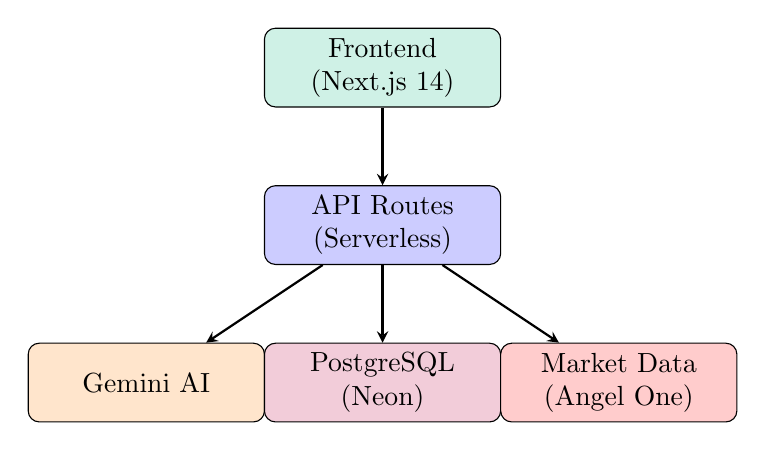
\begin{tikzpicture}[
    box/.style={draw, rounded corners, minimum width=3cm, minimum height=1cm, align=center},
    arrow/.style={->, thick, >=stealth}
]
    % Frontend
    \node[box, fill=primary!20] (frontend) at (0,4) {Frontend\\(Next.js 14)};
    
    % API Layer
    \node[box, fill=blue!20] (api) at (0,2) {API Routes\\(Serverless)};
    
    % Services
    \node[box, fill=orange!20] (ai) at (-3,0) {Gemini AI};
    \node[box, fill=purple!20] (db) at (0,0) {PostgreSQL\\(Neon)};
    \node[box, fill=red!20] (market) at (3,0) {Market Data\\(Angel One)};
    
    % Arrows
    \draw[arrow] (frontend) -- (api);
    \draw[arrow] (api) -- (ai);
    \draw[arrow] (api) -- (db);
    \draw[arrow] (api) -- (market);
\end{tikzpicture}
\end{center}

\subsection{Technology Stack}

\begin{techbox}[Frontend Technologies]
\begin{tabularx}{\textwidth}{lX}
    \textbf{Framework} & Next.js 14 with App Router \\
    \textbf{Language} & TypeScript (strict mode) \\
    \textbf{Styling} & Tailwind CSS with custom design system \\
    \textbf{Charts} & Recharts for interactive visualizations \\
    \textbf{Icons} & Lucide React icon library \\
    \textbf{State} & React hooks with server components \\
\end{tabularx}
\end{techbox}

\begin{techbox}[Backend Technologies]
\begin{tabularx}{\textwidth}{lX}
    \textbf{Runtime} & Node.js with TypeScript \\
    \textbf{API} & Next.js API Routes (Serverless) \\
    \textbf{ORM} & Prisma with type-safe queries \\
    \textbf{Authentication} & NextAuth.js v4 \\
    \textbf{Password Hashing} & bcryptjs \\
    \textbf{Email} & Nodemailer with Gmail SMTP \\
\end{tabularx}
\end{techbox}

\begin{techbox}[Database \& Infrastructure]
\begin{tabularx}{\textwidth}{lX}
    \textbf{Database} & PostgreSQL (Neon - Serverless) \\
    \textbf{Hosting} & Vercel (Edge Network) \\
    \textbf{Domain} & istocks.codes (Custom SSL) \\
    \textbf{Cron Jobs} & Vercel Cron for scheduled updates \\
    \textbf{Version Control} & Git with GitHub \\
\end{tabularx}
\end{techbox}

\begin{techbox}[AI \& Data Processing]
\begin{tabularx}{\textwidth}{lX}
    \textbf{AI Model} & Google Gemini 2.5 Pro \\
    \textbf{AI SDK} & Vercel AI SDK \\
    \textbf{Market Data} & Angel One API \\
    \textbf{Technical Analysis} & technicalindicators library \\
    \textbf{Data Scripts} & Python for bulk processing \\
\end{tabularx}
\end{techbox}

\subsection{Database Schema}

Key entities in the database:

\begin{itemize}[leftmargin=*]
    \item \textbf{Stock:} Symbol, name, exchange, price data
    \item \textbf{StockPrice:} OHLCV data with 20+ technical indicators
    \item \textbf{User:} Authentication and profile data
    \item \textbf{Account/Session:} OAuth and session management
    \item \textbf{Strategy:} User-created trading strategies
    \item \textbf{Backtest:} Strategy backtesting results
    \item \textbf{ChatSession/ChatMessage:} Conversational history
\end{itemize}

% ========== API REFERENCE ==========
\section{API Endpoints}

\begin{table}[h]
\centering
\begin{tabularx}{\textwidth}{llX}
\toprule
\textbf{Method} & \textbf{Endpoint} & \textbf{Description} \\
\midrule
POST & /api/chat & AI chatbot interactions \\
GET & /api/stocks & List all available stocks \\
GET & /api/stocks/[symbol] & Get stock details and prices \\
POST & /api/stocks/[symbol]/analyze & AI analysis for specific stock \\
GET & /api/sangraha & List all strategies \\
POST & /api/sangraha & Create new strategy \\
POST & /api/sangraha/[id]/backtest & Run backtest on strategy \\
POST & /api/sangraha/[id]/fork & Fork a public strategy \\
POST & /api/auth/signup & User registration \\
GET/POST & /api/auth/[...nextauth] & NextAuth handlers \\
GET & /api/cron/update-stocks & Scheduled stock data update \\
\bottomrule
\end{tabularx}
\caption{Core API Endpoints}
\end{table}

% ========== SECURITY ==========
\section{Security Implementation}

\begin{featurebox}[Security Measures]
\begin{itemize}[leftmargin=*]
    \item \textbf{Password Security:} bcrypt hashing with salt rounds
    \item \textbf{OAuth 2.0:} Secure Google authentication flow
    \item \textbf{Session Management:} Secure JWT tokens with NextAuth
    \item \textbf{HTTPS:} SSL/TLS encryption on all endpoints
    \item \textbf{Input Validation:} Zod schema validation on all inputs
    \item \textbf{SQL Injection Prevention:} Prisma's parameterized queries
    \item \textbf{Environment Variables:} Secrets stored in Vercel
\end{itemize}
\end{featurebox}

% ========== FUTURE ROADMAP ==========
\section{Future Roadmap \& Suggestions}

\subsection{Short-Term Enhancements}

\begin{enumerate}[leftmargin=*]
    \item \textbf{Portfolio Tracking:} Allow users to create and track virtual portfolios
    \item \textbf{Price Alerts:} Push notifications for price movements
    \item \textbf{Watchlists:} Personal stock watchlists with quick access
    \item \textbf{Market News Integration:} Real-time financial news feed
    \item \textbf{Export Reports:} PDF/Excel export of analysis
\end{enumerate}

\subsection{Medium-Term Features}

\begin{enumerate}[leftmargin=*]
    \item \textbf{Paper Trading:} Simulated trading with virtual money
    \item \textbf{Strategy Marketplace:} Paid premium strategies
    \item \textbf{Social Features:} Follow traders, share insights
    \item \textbf{Options Analysis:} Options chain and greeks calculator
    \item \textbf{Multi-Exchange Support:} Add MCX, commodity markets
\end{enumerate}

\subsection{Long-Term Vision}

\begin{enumerate}[leftmargin=*]
    \item \textbf{Mobile Application:} Native iOS/Android apps
    \item \textbf{Broker Integration:} Direct trading via broker APIs
    \item \textbf{ML-Based Predictions:} Custom trained models for price prediction
    \item \textbf{Voice Assistant:} Voice-based stock queries
    \item \textbf{API for Developers:} Public API for third-party apps
\end{enumerate}

\subsection{Infrastructure Recommendations}

\begin{itemize}[leftmargin=*]
    \item \textbf{AWS Migration:} Move compute-intensive backtesting to AWS Lambda/EC2
    \item \textbf{Redis Cache:} Add caching layer for frequently accessed data
    \item \textbf{CDN:} Utilize AWS CloudFront for static assets
    \item \textbf{Message Queue:} SQS for async processing of large backtests
    \item \textbf{Monitoring:} Implement AWS CloudWatch for observability
\end{itemize}

% ========== DEPLOYMENT ==========
\section{Deployment \& DevOps}

\begin{techbox}[Current Infrastructure]
\begin{tabularx}{\textwidth}{lX}
    \textbf{Platform} & Vercel (Hobby Plan) \\
    \textbf{Database} & Neon PostgreSQL (Serverless) \\
    \textbf{Domain} & istocks.codes (Cloudflare DNS) \\
    \textbf{CI/CD} & GitHub Actions + Vercel Auto-Deploy \\
    \textbf{Monitoring} & Vercel Analytics \\
\end{tabularx}
\end{techbox}

\textbf{Deployment Flow:}
\begin{enumerate}[leftmargin=*]
    \item Push code to GitHub main branch
    \item Vercel automatically triggers build
    \item Prisma generates client during build
    \item Next.js compiles and optimizes
    \item Deploy to global edge network
\end{enumerate}

% ========== CONCLUSION ==========
\section{Conclusion}

iStocks represents a significant step forward in democratizing financial analysis for Indian retail investors. By combining the power of AI with real-time market data and an intuitive interface, the platform enables users to make more informed investment decisions.

The modular architecture and modern tech stack ensure scalability and maintainability as the platform grows. With the planned roadmap items, iStocks is positioned to become a comprehensive financial intelligence platform.

\vspace{1cm}

\begin{center}
\rule{0.4\textwidth}{0.5pt}
\end{center}

% ========== FOOTER ==========
\vfill

\begin{center}
    \textcolor{primary}{\Large\faChartLine}\\[0.5cm]
    {\large\textbf{iStocks}}\\[0.2cm]
    {\small Empowering Investors with AI}\\[1cm]
    
    \textcolor{textgray}{\small Live: \url{https://istocks.codes}}\\[0.3cm]
    \textcolor{textgray}{\small GitHub: \url{https://github.com/i24hour/istocks-p}}
\end{center}

\vspace{2cm}

\begin{flushright}
    \textbf{CREATED BY: Priyanshu}
\end{flushright}

\end{document}
